\subsubsection{Language}

	At the beginning, the first choice for the project was C++ for coding the software. This is for simple reasons, C++ allows to create in most of the cases better software.  Moreover it has several complete graphical libraries, like Qt or SFML, so it's easy to create the graphical interface that we need for the project.

\subsubsection{Software}

	The choice of the sofware solution is fixed so that it can be used to develop the project. The coding part will be realized on Microsoft visual studio 2013, and the version manager will be Git. These two software are often used in the industry so it's better to be familiar with them.
For the bibliography, Zotero will be used, it allows the creation of .bib, the bibliographic format that will be used to write the reports.

\subsubsection{Grid'5000}

	Grid'5000 is a cluster of computers shared between many sites in France, it links a lot of computer of different centers of research. In addition of good CPU, some of this machines have a NVIDIA Tesla GPU that could be used to parallelize the MCTS. Of Course, use of this cluster will require some specific parallelization that will be presented in the next part.

\subsubsection{Parallelization}

\paragraph{Multi cores parrelization}\mbox{}\\\mbox{}\\
%prateek work
	OpenMp is a very simple and efficient API\footnote{Application Programming Interface} that supports parallelization. It consists some pre-compilation instructions, with only a few lines of code. It allows to obtain a parallel version of the algorithm. As it can be seen in the figure \ref{fig:OpenMp}, it uses a large part of shared memory which allows a quick and efficient communication between the different threads. But it's not designed for using a cluster of computers, because the memory access will not be efficiant for computers which are far away. But there is a method to avoid this problem that is addressed later.
\begin{figure}[!h] 
\centerline{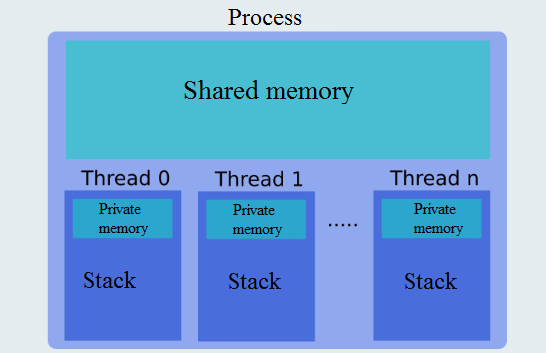
\includegraphics[scale=0.50]{3_Software_considered/MultithreadingMP_boost_Visual_MPI_5000_Zotero_Project_Baptiste/OpenMP}}
   \caption{\label{étiquette} OpenMp : memory management}
\label{fig:OpenMp}
\end{figure}
\newpage
\paragraph{Computer parallelization}\mbox{}\\\mbox{}\\

	MPI is a more complex method of parallelization than openMp but it is more complete, in addition to use several cores on a single machine, MPI can also be used  to designe the software that uses a cluster of machines. As it can be seen in the figure \ref{fig:MPI}, it doesn't use shared memory, all the data of the threads are duplicated at their creation. It uses signals to permit the communication between the threads. One of its advantages is that it makes possible to use multiple computers, as the data are duplicated there isn't the problem of time to access the memory. But attention is to be paid for the cost of communication between the threads, if  too many  signals are used, there will be loss of time that was gained using the parallelization. It's  adapted for  tree parallelization, because the only things to be done is to duplicate the data at the beginning and return the result at the end of the assign time.

\begin{figure}[!h] 
\centerline{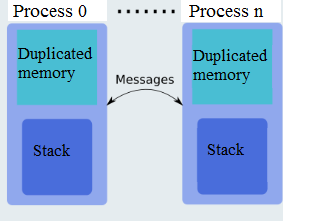
\includegraphics[scale=0.85]{3_Software_considered/MultithreadingMP_boost_Visual_MPI_5000_Zotero_Project_Baptiste/MPI}}
   \caption{\label{étiquette} MPI : memory management}
\label{fig:MPI}
\end{figure}


\paragraph{Hybrid parallelization}\mbox{}\\\mbox{}\\

	As it  is seen that openMp and MPI have  their respective pros and cons, but problems can be reduced by using both. That means MPI can be used to dispatch the work onto the different computers and successively  openMp can be used to divide it on different threads of each machine. This can permit to use together multiple parallelization strategy like tree between the machine and leaf or root on each machine. Also, it reduces the manual treatment that is to be defined in the code to manage the threads. It also means  that as the interaction between the threads is reduced, so maximum of the parallel code is kept.

\paragraph{Boost Library}\mbox{}\\\mbox{}\\

	Boost is a classical library of C++ which permits the management of threads, amongst other things.Bbasically, it can only be  used for one computer but it also contains a socket handling which should easily permit a parallelization between several machines. The library is simple to use and complete. Also, it holds tools for graph modelisation that can improve a lot  of efficiency of the algorithms.

\paragraph{GPU implementation}\mbox{}\\\mbox{}\\

	During the research,it was observed that efficiancy of  MCTS algorithms improved by using GPU.As Kamil Rocki said in his thesis "Large Scale Monte Carlo Tree Search on GPU"  \cite{GPU} : one GPU's performance is equivalent to 50 CPU threads. But this implementation has some defaults, in fact that Gpu possess very less cache memory, so if the data model is too big the parallelization will be inefficient. Also the trees that it creates will be less deep than those of a CPU, but when a CPU can develop two branches, a GPU will be developing hundreds of branches simultaneously. Another thing that is to be kept in mind is, a GPU can switch to another thread immediately without any cost of context switching. 

	Grid5000 has NVIDIA GPU, so one of the possibility is to use hybrid as it was described previously by using MPI (or boost library) and openAcc (an equivalent of openMp which allows to use GPU) or CUBA (a framework for GPU parallelization develop by NVIDIA). In this way  great trees will be developed and have a better solution compared with using only CPU, even if the trees will be less deep.